% %\documentclass[a4paper]{article}
% \documentclass[aps,amssymb,amsmath,superscriptaddress,nofootinbib]{revtex4-1}


% %% Language and font encodings
% \usepackage[english]{babel}
% \usepackage[utf8x]{inputenc}
% \usepackage[T1]{fontenc}


% %% Sets page size and margins
% \usepackage[a4paper,top=3cm,bottom=2cm,left=3cm,right=3cm,marginparwidth=1.75cm]{geometry}

% %% Useful packages
% \usepackage{amsmath}
% \usepackage{graphicx}
% \usepackage[colorinlistoftodos]{todonotes}
% \usepackage[colorlinks=true, allcolors=blue]{hyperref}
% \usepackage{xspace}
% \newcommand{\JJ}[1]{{\textcolor{red}{#1}}}
% \newcommand{\eg}{$\epsilon$-greedy\xspace}
% \newcommand{\bex}{Boltzmann exploration\xspace}

% \usepackage{physics}

% \begin{document}
% \title{Gauge selection as a multi-armed bandit problem}
% \author{Joshua Job}
% \affiliation{Department of Physics and Astronomy, University of Southern California, Los Angeles, California 90089, USA}
% \affiliation{Center for Quantum Information Science \& Technology, University of Southern California, Los Angeles, California 90089, USA}

% \author{Daniel Lidar}
% \affiliation{Department of Physics and Astronomy, University of Southern California, Los Angeles, California 90089, USA}
% \affiliation{Center for Quantum Information Science \& Technology, University of Southern California, Los Angeles, California 90089, USA}
% \affiliation{Department of Electrical Engineering, University of Southern California, Los Angeles, California 90089, USA}
% \affiliation{Department of Chemistry, University of Southern California, Los Angeles, California 90089, USA}

% \begin{abstract}

% \end{abstract}
% \maketitle

\section{Introduction}

We recast the gauge selection problem in quantum annealing as a multi-armed bandit (MAB) problem, discuss some of the possible methods of applying techniques from the field of bandit problems to gauge selection, and provide the results of applying these techniques on an existing ensemble of problems with a wide variety of difficulty for existing quantum annealers. Further, we discuss some of the intricacies with comparing the performance of MAB techniques with standard benchmarking methods for heuristic solvers in this space.

Quantum annealing has a wide variety of potential applications, including circuit fault diagnosis \cite{cfd_2017}, machine learning \cite{Amin:2016,Benedetti:2016oz,Adachi:2015qe,Biamonte:2016aa,higgs_qa}, and optimization \cite{Farhi:01,q108,speedup,hen:14f}. However, many applications require some form of minor embedding procedure, as in \cite{Adachi:2015qe,higgs_qa,vinci2015nested}, whether for basic utility or for error suppression, and all quantum annealers have a $Z_2$, or spin-reversal, symmetry over which qubit spin states (such as current direction in a flux qubit) is as a logical $\pm 1$. These symmetries in the map from logical to physical Hamiltonian are dubbed ``gauges'', and maps between them are dubbed ``gauge transformations'' \cite{q108}.

The problem of gauge selection has rarely been explored to date. After the idea of gauge-averaging was introduced in order to get systematic and reliable estimates of performance in Ref. \cite{q108}, the overwhelmingly common strategy is to simply select gauges at random and perform an average, and indeed has been used in essentially every benchmarking paper with quantum annealers, see Refs. \cite{q108,higgs_qa,hen:14f,King:2015zr,DW2000Q} and others. Work on attempting to learn higher quality gauges is largely confined to the performance estimator of Ref. \cite{perdomo:15a}, which unfortunately has proven in further (unpublished) work to be not very robust. \JJ{This is my understanding, I briefly discussed it at the Google party with Venturelli and he said it wasn't robust. Need a ref for ``private communication''?} 

In this work, we seek to more intelligently select gauges by recasting the problem in the language of multi-armed bandit (MAB) problems. The terminology comes from the colloquial saying referring to slot machine as ``one-armed bandits'' \cite{bayesian_bandit}. A MAB problem is essentially that of a slot machine with many arms, each arm providing some a priori unknown reward distribution (though the user may know some properties of the distribution(s), such as their support, density of high-reward arms, etc.). One's goal in solving a MAB problem is to get as much (possibly discounted) reward as possible over some time horizon (or at any given time). Equivalently, one can minimize the expected regret, namely the difference between the reward would have gotten if one had always selected the arm with highest expected reward and the rewards one actually observes.

MAB problems are extremely difficult to analyze and generally one requires many simplifying assumptions, such as looking at Robbins \cite{robbins1952} original 2-armed Bernoulli bandit or making assumptions about the distribution of expected rewards over the arms, as in Ref \cite{infinitebandits}. However, numerous heuristic algorithms with theoretical guarantees on expected loss are available, including $\epsilon$-greedy, Boltzmann exploration, Thompson sampling, upper-confidence bound (UCB)-family algorithms, and more \cite{infinitebandits,banditalgorithms,bayesian_bandit}.

Since gauges each have different output probability densities over states and one will generally need to draw many samples from one's quantum annealer in order to get reasonable numbers of states of interest (as has occurred thus far), one can clearly view each gauge as an arm and the gauge selection task as the task of minimizing regret. By recasting the problem of gauge selection in this way, we are able to apply the full history and machinery of MAB problems to the problem of gauge selection.

In the following, we will briefly give a more detailed description of gauges and gauge-averaging, discuss in more detail the previous work on the gauge selection problem, and follow with a description of some of the common MAB algorithms and how the special properties of gauge selection affect our choice of algorithms. Finally, we will apply some of these gauge algorithms to the problem of gauge selection in simulation and discuss in what contexts the MAB gauge selection method may yield significant benefits.

\section{Gauges, gauge-averaging, and gauge selection}

The notion of gauge symmetries was introduced in Ref. \cite{q108}. The physical Hamiltonian of the system corresponding to a given logical problem is generally non-unique, with many transformations (able to be applied efficiently) corresponding to an identical logical problem. 

This gauge freedom, under ideal circumstances, doesn't matter. If the quantum system is noiseless with infinite precision couplers (without control errors), then performing a spin-reversal transformation, for instance, by replacing every Z operator in the Hamiltonian with it's spin-reversed form for some ensemble of qubits, namely $\sigma_i^z\rightarrow \sigma_i^x\sigma_i^z\sigma_i^x = -\sigma_i^z$ for qubit $i$, will leave the output distribution of the quantum annealer invariant (provided one applies the inverse transformation to the output bitstrings). The same can be said for permuting the variables in a fully connected problem if you have a uniform minor embedding \cite{Venturelli:2015pi} (without uniform minor embeddings, one will of course anticipate some differences between permutation gauges). 

However, as shown in numerous studies, starting with \cite{q108}, gauges can have a significant variation in quality, as measured by the probability of success of the optimization problem (that is, the ground state probability of the annealer's output distribution). These variations in quality are a result of the systematic local biases, stray fields, and internal control errors (ICE) endemic to any analog quantum computing platform such as quantum annealing, or really any NISQ device lacking significant error correction. While one may, in principle, be able to train a model using reinforcement learning to guess high quality gauges directly from the Hamiltonian, since much of the gauge variation results from crosstalks and other properties which are problem Hamiltonian dependent, this may well prove impossible in practice, as one would have to have a very large number of problems with extremely large amounts of data for each for the training process to work. It may yet prove possible, but testing its feasibility will be left to future work.

The response of the quantum annealing community has been from the beginning to dismiss the variation over gauges as unwanted noise, and seek to generate more robust estimates of performance by simply averaging over many gauges. This of course makes sense if one seeks to perform some scaling analyses that hold up from processor generation to processor generation. One wouldn't want to declare a speedup that is driven by noise arising from poorly understood processes that you'll almost certainly be engineering away in future chips. However, there is evidence from running the same problem classes on successive generations of annealers that this simply isn't true --- even gauge-averaged results are affected significantly by changes in the underlying hardware architectures \cite{pokharel2017performance}. One can compare the performance shown in Ref \cite{q108} on random binary Ising problems with Ref \cite{speedup} on the same problems on a later generation of D-Wave quantum annealer, where the scaling improves even for the gauge-averaged data.

Gauge-averaging does improve robustness of performance estimates on a per-problem basis, but it may have less effect on central percentiles of the distribution over instances, so long as one's instance class is sufficiently unstructured (for instance, random Ising problems, as in \cite{speedup}). Moreover, if one seeks to use existing annealers to solve interesting problems then if one can improve performance at low cost, then one would be foolish not to do so.

\subsection{Prior work on gauge selection: the performance estimator}
To date, the only known work on intelligent selection of gauges, what we call ``the gauge selection problem'', is found in the work of Perdemo-Ortiz et. al. on their ``performance estimator'' \cite{perdomo:15a}. The basic notion of this work was to sample only a relative handful of times from each of an ensemble of gauges, and then pick the best one --- the meaning of ``best'' being whichever had the largest value of their performance estimator.

Their performance estimator was defined as the negative of the mean energy of the states with the lowest $\epsilon$ percent of energies returned in their trial runs, with $\epsilon$ a free parameter to be tuned. The negative of the energy is taken so that the performance estimator is like a score function to be maximized. Ref. \cite{perdomo:15a} suggested that values of $\epsilon$ of $1-2\%$ were optimal.

Perdemo-Ortiz et. al. restricted their tests to only two instances, preselected for hardness. They demonstrated that for these problems there was reasonably good correlation between the best set of five gauges selected via this method and the highest quality gauges in their tests. One could then expect significant improvements in average success probability for the two instances, with performance improvements of up to an order of magnitude possible for the hardest problem they considered. Nevertheless, restricting themselves to only two instances left their claims for improvement on relatively shaky ground, and it has turned out that their performance estimator was not robust in other problem domains or other problems.

Nevertheless, their basic idea was likely a good one --- performing an estimate of the average energy observed among the highest quality solutions and greedily choosing to run only a small set of gauges that performed the best on that metric is actually broadly comparable to $\epsilon$-greedy approaches for MABs, which we will discuss in our review of MAB algorithms in the next section. And their insight that we should seek to exploit the idiosyncracies of our processors as best we can is an important one and served as part of the inspiration for the current chapter.

\section{Multi-Armed Bandits, their algorithms, and the MAB properties of the gauge selection problem}
As discussed in the introduction, MABs typically involve some finite number of arms with unknown reward distributions, and the task of the learner is to maximize reward or minimize regret over some time horizon. Typically, researchers take the reward distributions to have some known range of support, with the most common choice being Bernoulli distributed rewards $(0,1)$, which is amenable to analysis and proofs concerning the expected regret \cite{banditalgorithms,bayesian_bandit}.

\subsection{Gauge selection as a bandit problem}
The gauge selection problem is somewhat unusual in the field of bandits. First and foremost, the number of arms is extremely large --- spin-reversal transformations (SRTs) alone compose $2^N$ transformations for $N$ qubits. Moreover, if one is embedding a fully connected problem on $N_L$ qubits, it would involve $N_L!$ permutation transformations as well which combine multiplicatively, and that's for only a single minor embedding, of which one can readily construct many. In typical MAB contexts, the number of arms is taken to be finite and relatively small by comparison to the interesting time horizon whereas in our context the number of gauges/arms is effectively infinite.

In addition, the gauges (arms) do not directly provide us with a reward value. We are given states with associated energies, but in real life we generally do not know the ground state energy $E_0$ of the problem and, moreover, we generally do not take the raw energy as our reward --- being within $10\%$ of the ground state energy isn't $90\%$ as good as finding the minimizing configuration(s). Much as in the case of applying optimal stopping to these sorts of optimization problems by Vinci \& Lidar in Ref \cite{vinci2016optimally}, one has to first determine an interesting reward function $R(E)$ to translate the energies $E$ of returned states into a number which accurately represents the value of the state for one's purpose.

The most studied MAB reward distribution is the Bernoulli bandit, with rewards only being 0 and 1. If one's reward function $R(E)=1$ only for $E$ being the ground state energy, one recovers the Bernoulli bandit. We'll dub this the Bernoulli reward function. It is, however, largely inappropriate in the ``training'' of a MAB algorithm for our context --- quite generally we do not, in fact, know what the solution of our problem is in quantum annealing. If we knew, we wouldn't need the annealer. 

Another suggestive reward distribution, which we'll call the Gibbs-weighted (GW) reward function, is simply the negative of the energy weighted by it's Gibbs factor at a particular inverse temperature $\beta$ (a free parameter to be chosen). Given a list of the energies of every state observed $\vec{E}$, then the GW reward would be $R_{GW}(E)=\exp(-\beta E) E$. The GW reward function at $\beta=0$ is simply the energy, but as $\beta$ increases it places more and more weight on lower energies. \footnote{Some readers may be concerned by the unbounded nature of the weight factor here --- for even modest values of $\beta E$ the reward becomes far too large to directly represent in floating point. One can simply apply a global rescaling factor to all rewards, such as dividing by $\exp(-beta E_{min})$ for $E_{min}$ being the smallest observed energy from any arm. Since it's a global factor across all arms, it doesn't effect anything about their relative rewards, and makes any numerical errors only occur in states with high energies and correspondingly very small weights.} For our study below, we will be using the simplest reward function for the MAB algorithm in this family, namely the $\beta=0$, $R(E)=E$ (or more accurately $\abs{E}$ since typically $E<0$ and we are solving a minimization problem).

One can think of any number of reward functions to use, but these two broadly meet the features one would expect of an interesting reward functions. In real world applications, one would need to take care to define a truly meaningful reward function for the task at hand (in sampling applications, for instance, one may reward variety of solutions). This is very similar to the problem of defining costs and rewards in the optimal stopping context, discussed in Ref \cite{vinci2016optimally}.

Finally, one other significant difference is that in gauge selection one may not have a finite, known time horizon over which one seeks to maximize reward. The horizon may discount future rewards, or have a resource budget \cite{budgetedthompsonbandits,infinitelybudgetedbandits}, or involve some profitability criterion as in optimal stopping contexts. For our purposes, we will primarily focus on the anytime case. This is largely because, while optimal stopping profitability criteria or budgeted bandits are likely to be the most useful, the former are also fairly unstudied in the bandit literature and both would require extremely careful reward and cost models that are surely problem/field dependent.

In summary, the gauge selection problem is an infinitely many-armed bandit with bounded but application specific reward functions/distributions and application specific time horizons. A final wrinkle of this description is that in reality we have a restless bandit \cite{whittle1988restless}, where the reward distributions change over time (due to things like $1/f$ noise). However, we'll ignore this for our purposes here since we have limited throughput in our annealers and the variations are relatively small over the short timescales that are realistic in this case considering (less than an hour).

\subsection{Algorithms for many-armed bandits}
In this section, we will review some of the chief algorithms used in solving bandit problems in general, and particularly those that apply to our case of many-armed bandits.

We'll review terminology and define some of our symbols, we will borrow most of our notation from Kuleshov \& Precup \cite{banditalgorithms}, which makes an extensive overview of bandit algorithms and their performance. We will merely summarize the interesting results applicable to gauge selection here. Assume we have $K$ arms, represented by distributions $\{D_i\}$ with means $\{\mu_i\}$ and variances $\{\sigma_i^2\}$. At each timestep $t$ the player selects arm $j(t)$ and gets a reward $r(t)\sim D_{j(t)}$. The task of a MAB algorithm is to select $j(t)$ base on observed rewards $\{r(t)\}$. A proof from Ref \cite{lai1985asymptotically} demonstrated that regret for bandit algorithms has to scale at least logarithmically with the time horizon, ie regret is at least $\Omega(\log(T))$.

We will discuss four basic types of algorithms: $\epsilon$-greedy, Boltzmann exploration, upper-confidence bound (UCB), and Thompson sampling, and what they imply for gauge selection. Only one, UCB, has a fully detailed mathematical extension to the many/infinitely-armed bandit case with regret bounds, however that same extension can readily be adapted to the other algorithms.

\subsubsection{$\epsilon$-greedy}
The \eg strategy is dead simple: choose the arm with the highest empirical mean reward, but with probability $0<\epsilon<1$ select another arm at random. This algorithm has a linear regret bound with constant $\epsilon$ (of course, as $\epsilon$ of the time the algorithm ignores all accumulated information) and can be thought of the simplest extension gauge-averaging. Indeed, $\epsilon$ of the time gauges are selected exactly as with gauge-averaging, while $1-\epsilon$ of the time the observed best gauge is played. Reducing $\epsilon$ with time yields a poly-logarithmic bound on regret, though this wasn't found to be practically useful in Ref \cite{vermorel2005multi}. %We can and will, however, readily test it on our dataset of gauges.

\subsubsection{Boltzmann exploration}
Boltzmann exploration keeps track of the empirical mean rewards $s_i$, and then samples arms according to their softmax distribution, namely \[p_j(t)\propto\exp(-s_i/\tau)\] with a temperature parameter $\tau$. Much like the Boltzmann-weighted reward function's inverse temperature $\beta$, modifying $\tau$ can greatly alter the behavior of the algorithm. In this case, $\tau\rightarrow\infty$ takes the algorithm to standard gauge-averaging while $\tau\rightarrow 0$ shifts to a purely greedy strategy. 

One should take into account the magnitude of the expected rewards $s_i$ when determining $\tau$, much as one does when determining a schedule of temperatures in parallel tempering or simulated annealing. If rewards are bounded between 0 and 1, as in the Bernoulli reward mechanism, smaller values of $\tau$ should be used as compared to the generally very large weights from the Gibbs-weighted reward function. A natural method would be to normalize the reward functions so their maximum is $1$ and scale $\tau$ accordingly. 

It was found in Ref \cite{vermorel2005multi} that scaling $\tau$ down with temperature in practice yields no benefits even though it allows the derivation of a poly-logarithmic bound on regret. %As with \eg, however, we will test if it has practical utility.

\subsubsection{Upper-confidence bound (UCB)}
UCB algorithms are not merely a single algorithm, but a broad family. They enable some of the tightest and most rigorous bounds on regret available for bandit problems \cite{infinitebandits,banditalgorithms}. The essence of UCB algorithms, as the name suggests, is to take account of both the empirical rewards $s_i$ and empirical variances $v_i=\sigma_i^2$ ($\sigma_i$ here representing the standard deviation, not to be confused with one of the Pauli matrices) of each arm. One then effectively estimates an upper bound on the expected reward of each arm, mixed with an exploration function, and optimistically select the arm with the greatest upper bound. In the case of arms of similar empirical mean but different variances, this algorithm in essence assumes that the arm with the biggest variance is the one with the best real performance.

More rigorously, we will hear use the UCB-V algorithm, and follow the notation in Ref \cite{infinitebandits}, adjusted to match previous definitions. 

Define a non-decreasing sequence of numbers $\mathcal{E}_t$, indexed by the round of arm selection, which we may call the exploration sequence. Let $k_i$ be the number of times arm $i$ has been pulled up to the current round. Then at each round of arm selection, choose whichever arm maximizes the value of $B_i(t)$ where \[B_i(t)=s_i+\sqrt{\frac{2v_i\mathcal{E}_t}{k_i}}+\frac{3\mathcal{E}_t}{k_i}\]

As one can see, arms that have rarely been pulled get a bonus from the exploration sequence and from large variance, but as they are pulled more often $B_i(t)$ converges toward the expected reward $s_i$. The UCB-V algorithm was proven to have logarithmic regret.

An extension to the case of infinitely many armed bandits, as in the real gauge-selection problem, was introduced in Ref \cite{infinitebandits}. One variant, UCB-V($\infty)$ was appropriate for the finite horizon case, wherein one essentially selects an ensemble of arms $K$ at the start and then runs UCB-V on them. This algorithm achieves a bound linear in the number of rounds of play and proportional to $K^{1/\beta}$ where here $\beta$ arises from an assumption that the fraction of all arms with expected reward within $\epsilon$ of optimal scales like $\epsilon^\beta$ for small $\epsilon$, that is Pr$(s^*-s_i<\epsilon) = \mathcal{O}(\epsilon^\beta)$, where $s^*$ denotes the maximum mean reward in the space of all arms. One is advised to pick a number of arms $K=n^{\beta/\max(\beta+1,2)}$ for time horizon $n$, yielding an algorithm the authors of Ref \cite{infinitebandits} dub UCB-F, for fixed horizon.

The second variant is an anytime algorithm called UCB-AIR, which essentially involves, for an assumed/known $\beta$, for which arms are selected according to the UCB-V algorithm and the pool of all arms is increased such that it is always as large or larger than $t^{\beta/\max(\beta+1,2)}$, a strategy dubbed the arm-increasing rule or AIR (hence UCB-AIR). The authors of Ref \cite{infinitebandits} show that at anytime the algorithm is bounded and scales with $C n^{\beta/\max(\beta+1,2)} \log^2(n)$ for a constant $C$ dependent on $\beta$.

The proof of the bounds on regret based on this assumption are difficult to extend to other algorithms, but we can take the advise of $UCB-F$ and $UCB-AIR$ as a rough guideline for the selection of the number of arms in all our algorithms. In essence, one wishes to have at least one near-optimal arm in one's ensemble, and by selecting ``enough'' arms (ie gauges) one will be able to assure this with reasonable probability. 

Thus, we will be able to compare our algorithms both for a fixed number of gauges selected in advance and with a dynamically increasing number of gauges to sample from with time. The parameter $\beta$, henceforth known as $\alpha$, so as to minimize confusion, is unknown. For convenience only, we will select $\alpha=2$, to ease analysis. $\mathcal{E}_t$ will be taken at the more conservative growth rate suggested in \cite{infinitebandits}, namely $\mathcal{E}_t=\log{t}$.

\subsubsection{Thompson sampling}
The final category of algorithm we will consider is also arguably the oldest --- Thompson sampling, named after William R. Thompson who introduced the basic idea in a paper in 1933 \cite{thompson1933}. This algorithm also goes by the name of the ``Bayesian control rule'', and was reintroduced after being largely ignored since its introduction in a paper published in 2010 extending it to arbitrary contexts, Ref \cite{bayesiancontrol}, which gave it this alternative name. Following an empirical investigation into its performance presented at NIPS in 2011, Ref \cite{chapelle2011empirical}, it has since been shown to be asymptotically optimal in general environments, Ref \cite{leike2016thompson}, and been used in reinforcement learning many times, as in Ref \cite{osband2016deep} where a bootstrap-based variant was used in deep Q-learning.

From a Bayesian perspective, all of the aforementioned algorithms are unfounded --- they use simple frequentist observed expectations, essentially arbitrary exploration sequences, and/or softmax weighting in order to determine the arm to play next. Thompson sampling in the bandit setting, by contrast, directly answers the question ``Which arm should I play to get maximum expected return?'' with the answer ``Whichever arm you think gives the maximum expected return.''

If one keeps a posterior density for the expected returns from each arm, then by drawing a single sample from each posterior one can directly answer which one has the maximum expected return and play that. The resulting play will occur with exactly the frequencies corresponding to the subjective beliefs of the player.

More systematically, assume that each arm $i$ begins with a prior density $p_i(r_i)$ and is updated via Bayes rule to $p_i(r_i(t)|\vec{r}_i)$, where $\vec{r}_i$ are the observed returns from arm $i$. Then Thompson sampling suggests that the next arm to play is found by sampling values from all arms $\vec{r}$ with $i$th element $r_i(t)\sim p_i(r_i(t)|\vec{r}_i)$ and $j(t)=\textnormal{ind} \max \vec{r}(t)$. This can be viewed as taking a sample from the posterior distribution for the identity of the arm with greatest average return.

One immediately sees that under initially diffuse priors Thompson sampling will explore and, as the number of observations grows, slowly converge onto the real expected reward of the arms, thereby moving toward exploitation of the knowledge gained by experience.

In the Bernoulli reward setting, expected return is merely the probability of observing a reward from an arm. The natural prior is the conjugate prior to the Bernoulli distribution, $Beta(\alpha,\beta)$ for some positive real parameters $\alpha$ and $\beta$. Common choices are the Jeffreys prior $Beta(1/2,1/2)$ and the uniform prior $Beta(1,1)$ (so named because it assigns equal probability to all values between $0$ and $1$). The posterior given $k_i$ arm pulls for arm $i$ and $r_i$ observations of the reward is, in general, $Beta(\alpha+r_i,\beta+k_i-r_i)$, as was seen in \ref{ch:benchmarking}. This closed form of the posterior is extremely convenient and motivates the choice of conjugate priors, as no computationally expensive MCMC algorithm is required to estimate the posterior densities.

This highlights a key issue with the Bernoulli reward function --- if one does not have the ground state energy of the problem Hamiltonian on hand one does not actually know whether to grade the observed states from one's quantum annealer as either $0$ or $1$. One could simply assume the minimum energy $E_{min}$ observed thus far is the ground state $E_0$, updating on the fly if one finds a lower energy. This poses little issue for the \eg and \bex algorithms, merely slowing down exploration of the gauge landscape and finding the true ground state, and only a modest problem for UCB algorithms, it undermines the conceptual foundation for Thompson sampling. If one is to keep a posterior density,one properly needs to take into account uncertainty in the observed rewards as they may be edited in the future.

Luckily, this problem is not so complex --- in the case of Bernoulli rewards, one effectively has two models --- one in which $E_{min}=E_0$ and one in which $E_{min}\neq E_0$. We can define for each gauge a prior $Dir(\alpha,\beta,\gamma)$ with the components, respectively, representing the probability of finding a state lower than the lowest observed state, finding the lowest observed state, and finding a state higher than the lowest observed state. Taking these as values indexed by gauge, we can then represent these components as a grand Dirichlet distribution $Dir(\vec{\alpha},\vec{\beta},\vec{gamma})$ with the marginal distribution $Dir(\sum_i \alpha,\sum_i \beta,\sum_i \gamma)$ representing our state of belief above the likelihood across all gauges of sampling a state less than, equal to, or above the current minimum observed state.

Defined as a sampling procedure, we then would sample a value from $Dir(\sum_i \alpha,\sum_i \beta)$ (the marginal distribution over the belief that our current minimum state is the true minimum) and with that probability then sample values for each gauge from $Dir(\alpha_i,\beta_i+\gamma_i)$ (if we got 0, ie we sampled that our current minimum is not the true minimum) or $Dir(\beta_i,\gamma_i)$ (if we got 1, ie we sampled that the current minimum was indeed the true minimum). We then merely define a prior over all these possibilities as in the case where we knew the ground state. Due to aforementioned discussions of biases and the difficulty of learning in the ideal case for small probability instances for priors other than Haldane, we may choose something like $Dir(1,0,0)$ as a prior density. This would lead to a belief for our finding the minimum state of $Dir(G,\sum_i x_i)$ for observations of the minimum state per gauge $x_i$ and number of gauges $G$. This distribution clearly induces significant exploration across gauges until we observe a number of putative successes much larger than the number of gauges. Of course, other choices could be made, and it is an open question which tends to the best outcomes in practice.

A similar, though less severe, problem arises in the case of the Gibbs-weighted reward function. In this case, it is simply the problem of choosing an appropriate prior. If the prior places too much weight on energies smaller than $E_{min}$, one will effectively wash away any differences between the weights, and the resulting sampling will be approximately uniform. One possibility is to assume that $E_{min}$ is the true ground state, though this may lead to overfitting and rapid convergence to a highly degenerate or unusually likely excited state. We do not investigate these issues in detail here.

\section{Methods}
To test the impact of applying MAB algorithms to gauge selection, we will employ a dataset constructed by Tameem Albash based on his logical planted instances with gadgets from Ref \cite{albash2018demonstration}. These instances are unique in that they have exhibited an optimal annealing time for the first time on D-Wave devices, and span a wide range of empirical difficulty spanning from $8e-6$ per trial on average to approximately $3e-3$ for the instances discussed here, a span of nearly $3000$ fold.

For our purposes here we are not concerned with optimal annealing times, but employ these for their wide range of difficulty. We extracted 13 problems from the 100 in the original dataset, which corresponded to problems the problems with index 1,2,5,10,15,20,30,40,50,60,70,80,90 when ranked from lowest probability of success to highest. This gives a good range of problems with varying hardness on which to run our MAB gauge selection techniques. We then run each of 100 gauges with 100 programming cycles each, each programming cycle with 1000 anneals, yielding a total of $10^7$ samples per problem, and $10^5$ per gauge.

To simulate the behavior of our algorithms, we take a bootstrap-like approach. When an algorithm chooses a gauge $g$, one of the 100 programming cycles for gauge $g$ from the device is used as the return distribution on which we calculate our rewards. This can be thought of as a kind of block bootstrap, as it maintains any correlations between the samples in a single programming cycle (should there be any).

For each algorithm, we will simulate 100 plays of the many-armed bandit gauge selection game for each instance, each game containing $10^4$ simulated programming cycles (each being a lever pull/gauge selection event). This way we will get detailed statistics on the behavior of the algorithm as a function of time for analysis. We will also attempt two variants of each algorithm: a fixed-arm version, in which we pin the number of arms to be 10,20,50, and 100 (sampled with replacement from the 100 gauges available), as well as the arm-increasing rule (AIR) variant in which the number of gauges is increased with time with $\alpha$ (formerly, $\beta$) of 2 chosen for convenience.

As for algorithm-specific parameters: 
\begin{itemize}
\item  \eg, we will use varying values of $\epsilon$, 0.01,0.02,0.05, 0.1, and 0.2.
\item Boltzmann sampling, we will be testing a variety of temperatures [0.1,0.2,0.5,1.,2.,5.,10.].
\item UCB, we will employ the standard schedule for $\mathcal{E}_t=\log(t)$.
\item Thompson sampling we will test our proposed prior of $Dir(1,0,0)$ as discussed above. Note, that uniquely among the algorithms here, this is arguably the only algorithm being run with a Bernoulli reward function, since the MAB algorithm is directly trying to maximize the likelihood of finding the ground state, while the other algorithms are running without any such goal, instead working to maximize average energy returned. The primary reason here is that while we typically do not know the minimum, Thompson sampling involves sampling the possibility that the ground state is lower than the lowest energy state observed.
\end{itemize}

A quick note regarding error estimation in this context. Due to computational constraints, here the 25th and 75th percentiles of the various performance metrics are typically plotted along with the mean and median, in order to give a rough picture of the variation from run to run.

\section{Results}

Here we will present a small subset of our full dataset, chosen to highlight some of it's key features.

First, just to give a general understanding of how one may plot the results, we have Figure \ref{fig:boltzmann_inst10_air}. There one can see plots of the cumulative number of successes against the number of simulated gauges, the ratio of the cumulative successes between the MAB algorithm and the blind algorithm, and that same ratio plotted against the cumulative number of successes. This last typically approaches an asymptotic value that shows the total benefit (in terms of sampling the success probability) of using the MAB algorithm vs the standard blind averaging. Here we see we can achieve very rapid rises to $\approx 2$x the rate of successes for most instances.

\begin{figure}
    % \centering
    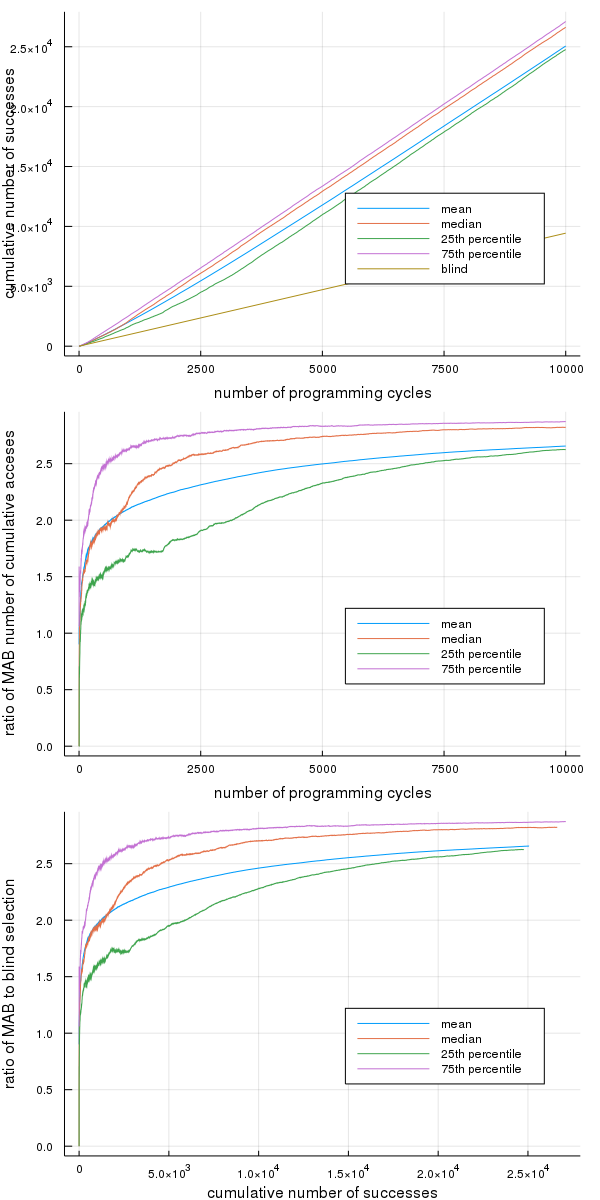
\includegraphics[width=0.7\columnwidth]{boltzmann_inst10_air.png}
    \caption{The basic types of fundamental plots --- The first panel shows cumulative number of true successes in the simulation as a function of the number of gauges, the second shows the ratio between said cumulative successes for the MAB algorithm (here Boltzmann with energy 1) to that which one would expect from randomly selecting gauges. And finally there is the third panel, showing the MAB-to-blind cumulative successes against the number of successes observed by that point. This latter is quite nice, in that the value at any given point is an estimate of the magnitude of the benefit (the improvement in the rate of successes) of running the MAB. This particular plot is instance 10, the 60th percentile, using Boltzmann sampling at $\beta=1$ using an adjustable number of arms.}
    \label{fig:boltzmann_inst10_air}
\end{figure}

We'll go algorithm by algorithm to give a flavor of their behavior as a function of their parameters and with the problem hardness. 

\subsection{\eg}

\eg is a dead-simple algorithm, with only one free parameter in the anytime case, namely $\epsilon$. I present \ref{fig:epsilon_inst1_air_eps_comp} and \ref{fig:epsilon_inst13_air_eps_comp} which represent the equivalent of the 5th and 90th percentiles of instances, and are fairly representative. As one can see, the looser $\epsilon=0.1$ tends to help the 25th percentile for the harder problem, there is very little difference for fairly easy problems. However, since $\epsilon=0.1$ can only reduce the number of successes per gauge on average by only $10\%$ from the maximum theoretical value, it is likely preferable in practice to use the looser value.

\begin{figure}
    % \centering
    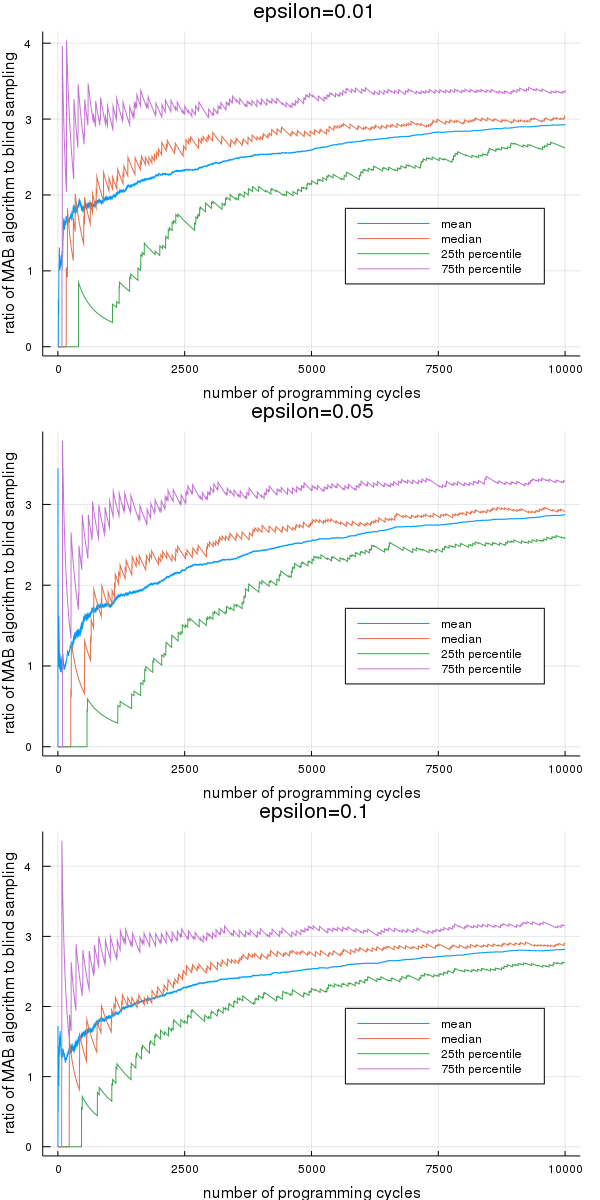
\includegraphics[width=0.7\columnwidth]{epsilon_inst1_air_eps_comp.png}
    \caption{Plot of ratio of MAB to blind cumulative success as a function of the number of programming cycles for the instance representing the 5th percentile of the dataset for $\epsilon=\{0.01,0.05,0.1\}$. We see a significant improvement for the 25th percentile of trials, though not a very large difference in the scaling of each algorithm individually.}
    \label{fig:epsilon_inst1_air_eps_comp}
\end{figure}

\begin{figure}
    % \centering
    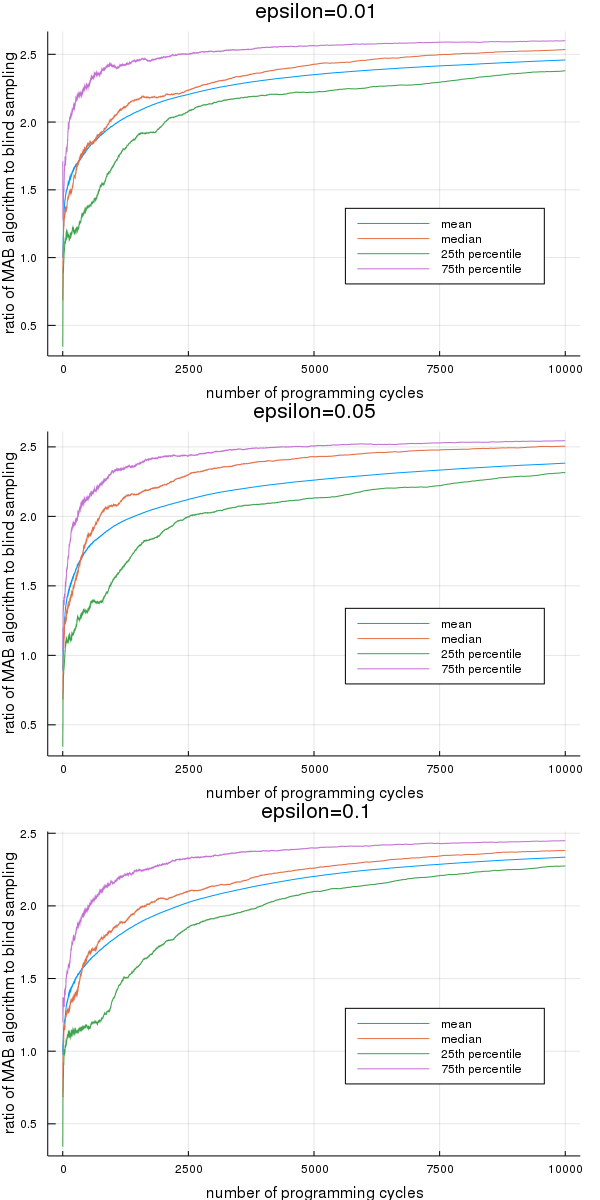
\includegraphics[width=0.7\columnwidth]{epsilon_inst13_air_eps_comp.png}
    \caption{Plot of ratio of MAB to blind cumulative success as a function of the number of programming cycles for the instance representing the 90th percentile of the dataset for $\epsilon=\{0.01,0.05,0.1\}$. We see fairly little variation, as easy instances have such high probabilities tend to have somewhat less variation in relative probability magnitudes than harder instances.}
    \label{fig:epsilon_inst13_air_eps_comp}
\end{figure}

Finally, we'll provide a representation of the MAB to blind ratio for the average trial for $\epsilon=0.1$ (given our conversation above), just to give a rough sense of how performance varies with hardness percentile of the underlying problem, see Figure \ref{fig:epsilon_air_mabratio_mean}.

\begin{figure}
    % \centering
    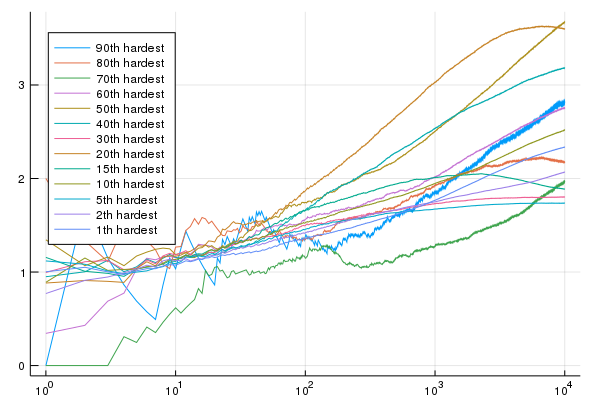
\includegraphics[width=0.8\columnwidth]{epsilon_air_mabratio_mean.png}
    \caption{Plot of the mean ratio over repeated trials of MAB to blind cumulative success as a function of the number of programming cycles for the 13 problems discussed here for \eg.}
    \label{fig:epsilon_air_mabratio_mean}
\end{figure}

\subsection{Boltzmann sampling}

In our study, we find that Boltzmann sampling generally performs reasonably well except for the very hardest problems, which seem to suffer from over-specialization to suboptimal gauges, but which have at least some probability of finding a success. However for those hardest problems, increasing temperature results in improved performance, in particular it largely prevents a large ($>25\%$) of trials from performing worse than a blind guess as they do at lower temperatures, though it may cause worse performance on easier problems. For a representative example of the behavior for different temperatures, see figures \ref{fig:boltzmann_inst3_air_eps_comp} and \ref{fig:boltzmann_inst1_air_eps_comp}.

There is little to additional to say about Boltzmann sampling, but we will provide some additional comments in some cross-algorithmic comparisons below. And we will also reproduce an equivalent of figure \ref{fig:epsilon_air_mabratio_mean} in figure \ref{fig:boltzmann_air_mabratio_mean}.

\begin{figure}
    % \centering
    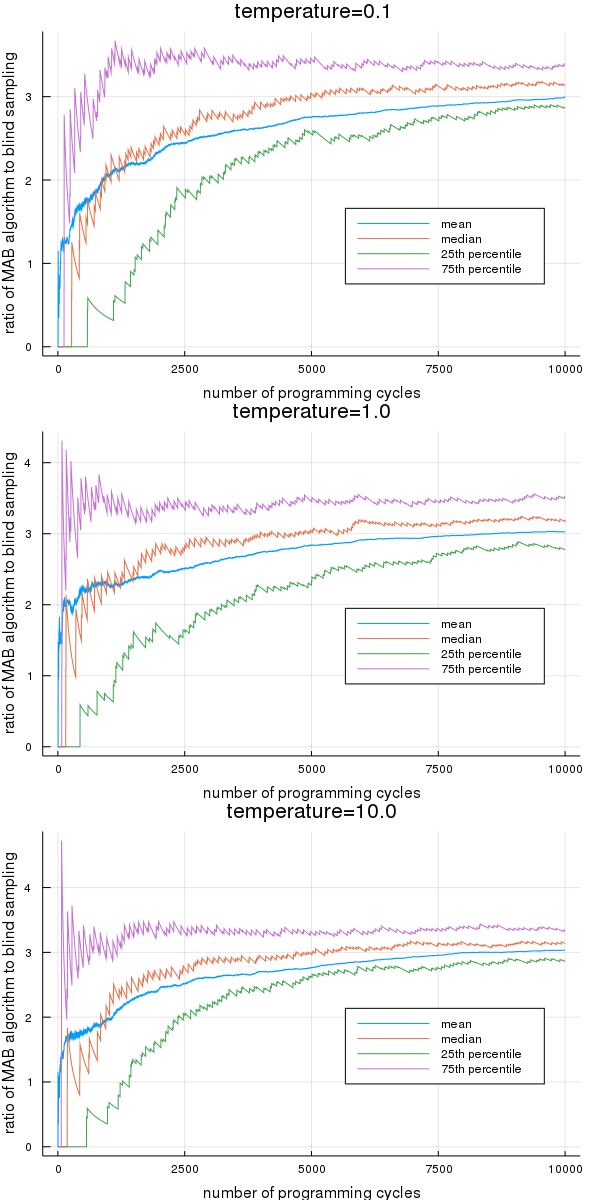
\includegraphics[width=0.8\columnwidth]{boltzmann_inst1_air_eps_comp.png}
    \caption{Plot of the mean ratio over repeated trials of MAB to blind cumulative success as a function of the number of programming cycles for the instance equal to the 5th percentile in probability of success of the instance class. We see similar performance, but some small degradation as we go to higher temperatures.}
    \label{fig:boltzmann_inst1_air_eps_comp}
\end{figure}

\begin{figure}
    % \centering
    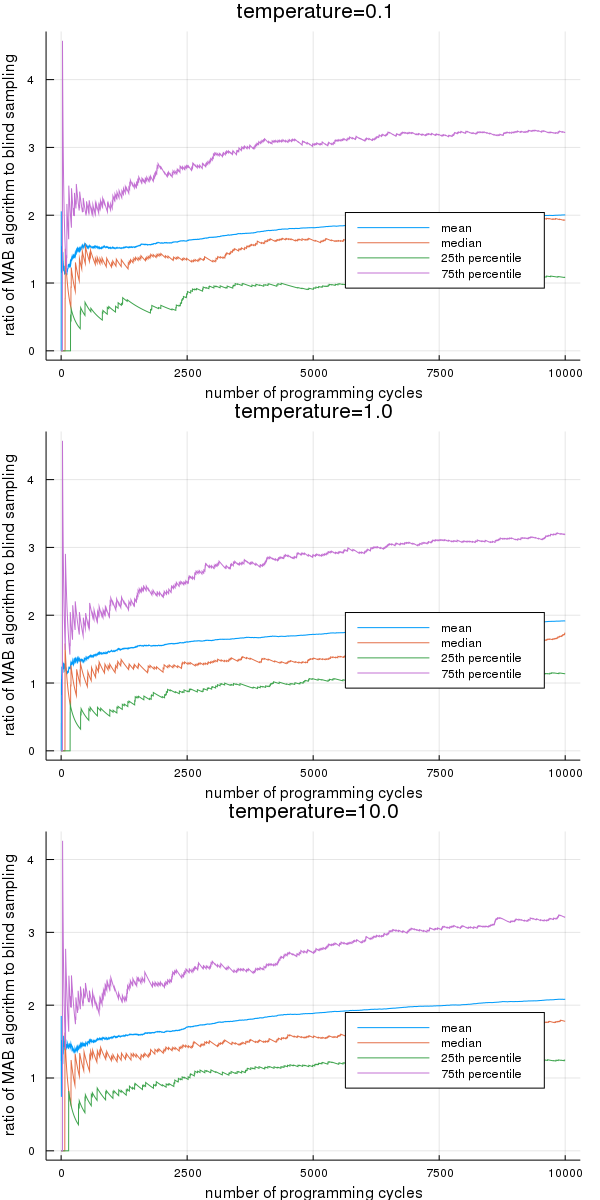
\includegraphics[width=0.8\columnwidth]{boltzmann_inst3_air_eps_comp.png}
    \caption{Plot of the mean ratio over repeated trials of MAB to blind cumulative success as a function of the number of programming cycles for the hardest instance of the instance class, and see an improvement in performance as temperature increases. By increasing temperature, performance broadly improves, in particular the 25th percentile more rapidly moves above breakeven (ie $1$).}
    \label{fig:boltzmann_inst3_air_eps_comp}
\end{figure}

\begin{figure}
    % \centering
    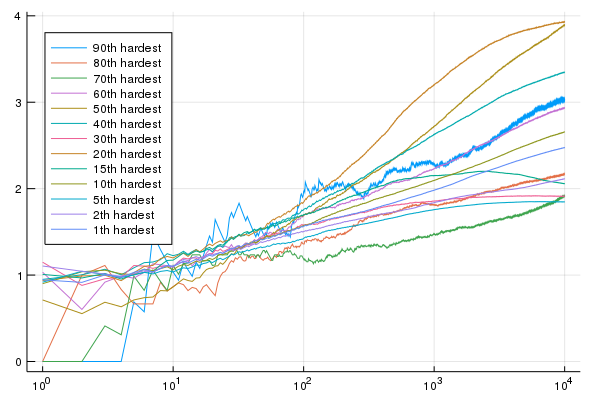
\includegraphics[width=0.8\columnwidth]{boltzmann_air_mabratio_mean.png}
    \caption{Plot of the mean ratio over repeated trials of MAB to blind cumulative success as a function of the number of programming cycles for the 13 problems discussed here for Boltzmann sampling at temperature$=1$.}
    \label{fig:boltzmann_air_mabratio_mean}
\end{figure}

\section{UCB}

Interestingly, of all the algorithms, UCB performed the worst. This may be a result of a suboptimal schedule for $\matchal{E}_t$ (here $log(t)$) but this seems to be  very common choice in the literature. UCB occasionally reached high rates of return, but also had a high probability of performing very poorly. This may be due to properties of the underlying distribution of energies, which in our experience tend to be overdispersed (see some of the supplemental information, for instance, in Ref \cite{higgs_qa}). Here we will simply reproduce a few figures similar to previous sections --- at least based on this provisional evidence, UCB may not be the best algorithm for the task of gauge selection. More work is needed to discern exactly why this is the case.

\begin{figure}
    % \centering
    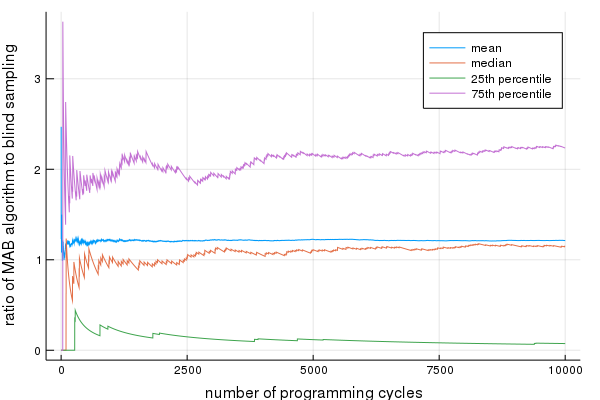
\includegraphics[width=0.8\columnwidth]{ucb_inst3_air.png}
    \caption{Plot of the mean ratio over repeated trials of MAB using UCB to blind cumulative success as a function of the number of programming cycles for the hardest instance of the instance class. Performance is widely overdispersed --- there is a significant chance of very high returns, but also very high probability of very poor returns, with the average case being unimpressive by comparison to other algorithms here.}
    \label{fig:boltzmann_inst3_air}
\end{figure}

\begin{figure}
    % \centering
    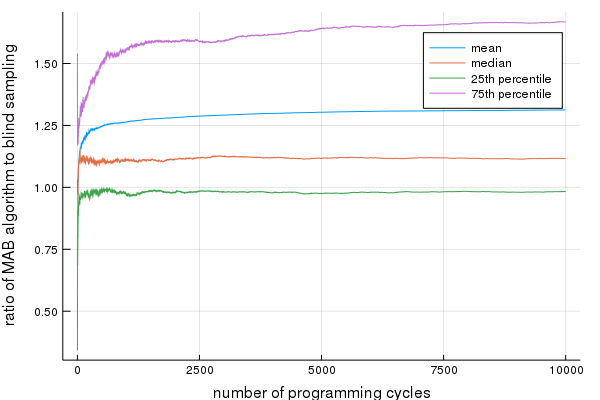
\includegraphics[width=0.8\columnwidth]{ucb_inst13_air.png}
    \caption{Plot of the mean ratio over repeated trials of MAB using UCB to blind cumulative success as a function of the number of programming cycles for the 10th easiest problem in the class. Compared to the same plot in Figure \ref{fig:epsilon_inst13_air_eps_comp}, for instance, performance is poor.}
    \label{fig:ucb_inst13_air}
\end{figure}

\begin{figure}
    % \centering
    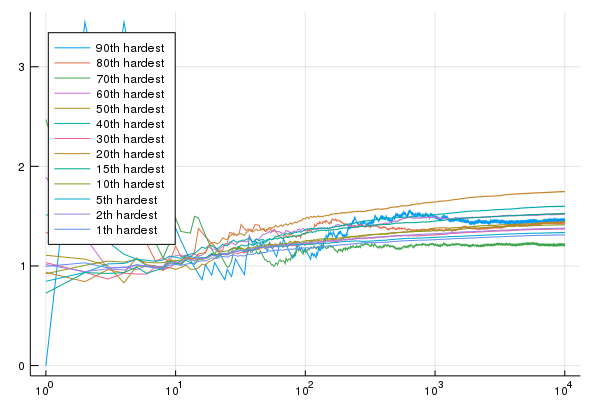
\includegraphics[width=0.8\columnwidth]{ucb_air_mabratio_mean.png}
    \caption{Plot of the mean ratio over repeated trials of MAB using UCB to blind cumulative success as a function of the number of programming cycles for the 13 problems discussed here. It is fairly clearly quite consistent but much worse, on the whole, than other algorithms we test here.}
    \label{fig:ucb_air_mabratio_mean}
\end{figure}

\subsection{Thompson sampling}

Thompson sampling performs broadly similar to Boltzmann sampling and \eg, but the cumulative return curves are almost universally much smoother and predictable, and reaches higher maximum returns than any other algorithm. Here, we reproduce the figures for the returns for the 5th percentile of instances \ref{fig:thompson_inst1_air}, the 20th percentile \ref{fig:thompson_inst6_air}, and the 90th \ref{fig:thompson_inst13_air}. The plot for the 5th percentile is especially interesting --- here, rather than the semi-greedy approach of \eg and Boltzmann sampling, we see that as the number of trials (and thus gauges being tested) increases, the algorithm essentially converges to close to random guessing. This is largely because the number of times we ever observe the ground state for that problem is very very low, and thus our prior $Beta(G,x)$ (for number of gauges $G$ and total observations of the lowest energy state thus far $x$) is strongly biased toward there being lower energy states.

However, by the time we look at the 20th percentile (or the 90th), the algorithm performs quite well and all curves (mean, median, 25th and 75th percentiles) rise smoothly. We plot the mean return for each instance, as before, in Figure \ref{fig:thompson_air_mabratio_mean}, seeing that it is competitive with the best algorithms tested before, and achieves the highest returns of any algorithm on a small set of instances.

\begin{figure}
    % \centering
    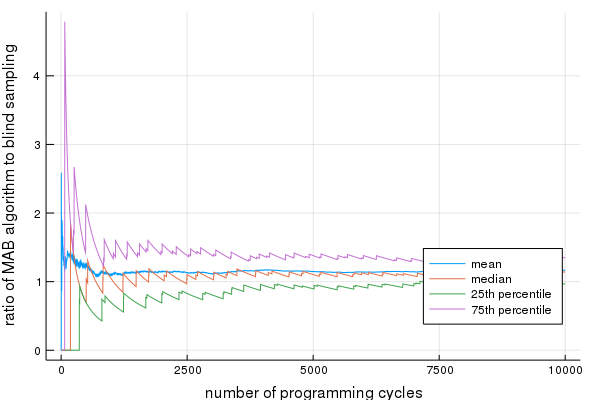
\includegraphics[width=0.8\columnwidth]{thompson_inst1_air.png}
    \caption{Plot of the mean ratio over repeated trials of MAB using UCB to blind cumulative success as a function of the number of programming cycles for the 5th hardest problem in the class. Performance collapses to blind guessing, as our prior density places significant prior probability that there are lower energy states so long as the number of ``arms'' in our bandit is larger than the number of successes.}
    \label{fig:thompson_inst1_air}
\end{figure}

\begin{figure}
    % \centering
    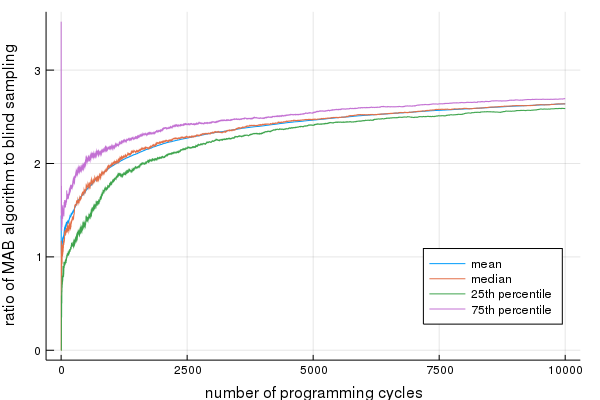
\includegraphics[width=0.8\columnwidth]{thompson_inst6_air.png}
    \caption{Plot of the mean ratio over repeated trials of MAB using UCB to blind cumulative success as a function of the number of programming cycles for the 20th hardest problem in the class. Performance now smoothly increases, in contrast to \ref{fig:thompson_inst1_air}.}
    \label{fig:thompson_inst6_air}
\end{figure}

\begin{figure}
    % \centering
    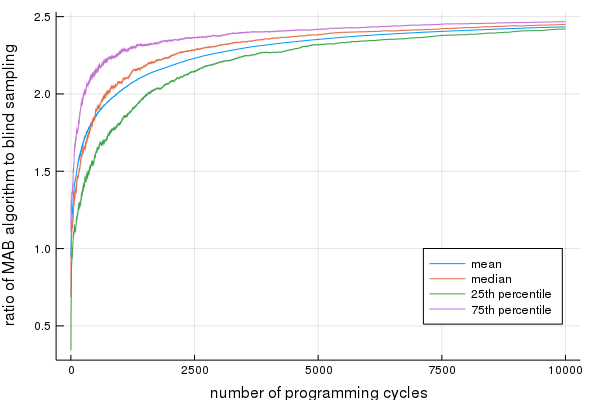
\includegraphics[width=0.8\columnwidth]{thompson_inst13_air.png}
    \caption{Plot of the mean ratio over repeated trials of MAB using UCB to blind cumulative success as a function of the number of programming cycles for the 10th easiest problem in the class. Performance is still reasonble, and again rises smoothly across the whole space.}
    \label{fig:thompson_inst13_air}
\end{figure}

\begin{figure}
    % \centering
    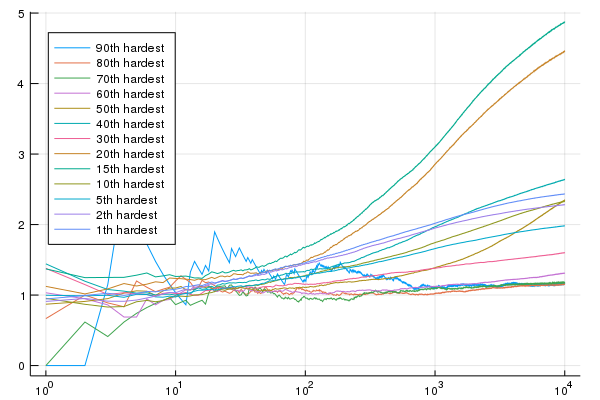
\includegraphics[width=0.8\columnwidth]{thompson_air_mabratio_mean.png}
    \caption{Plot of the mean ratio over repeated trials of MAB using Thompson sampling to blind cumulative success as a function of the number of programming cycles for the 13 problems discussed here. It is fairly clearly quite consistent, and actually reaches by far the highest rates of return for certain problems as compared with UCB, Boltzmann sampling, and \eg.}
    \label{fig:thompson_air_mabratio_mean}
\end{figure}

\subsection{Comparing different algorithms}
Here, we briefly address the question of ``which algorithm is `best'?''. Briefly, both for brevity and because this study simply isn't equipped to answer the question. As was seen in Chapter \ref{ch:benchmarking}, we need to think carefully about what we have learned here. And due to the small set of instances, the lack of complete optimization of the parameters of the algorithms, and limited (even though large) dataset, we simply can't make very strong claims here.

Provisionally, we can clearly eliminate UCB in this case. Comparing of the remaining three algorithms, we will simply plot a bar graph representing the maximum ratio of return from the MAB algorithm to that of blind guessing to give some indication of their relative performance in the end, in Figure \ref{fig:mean_max_return_comp}. Looking at the graph, we see that Thompson sampling generally performs worse than either \eg or Boltzmann sampling, with Boltzmann sampling narrowly outperforming \eg. Thus, we can very provisonally recommend Boltzmann sampling. However, much further study would be required before any dependable statements can be made.

\begin{figure}
    % \centering
    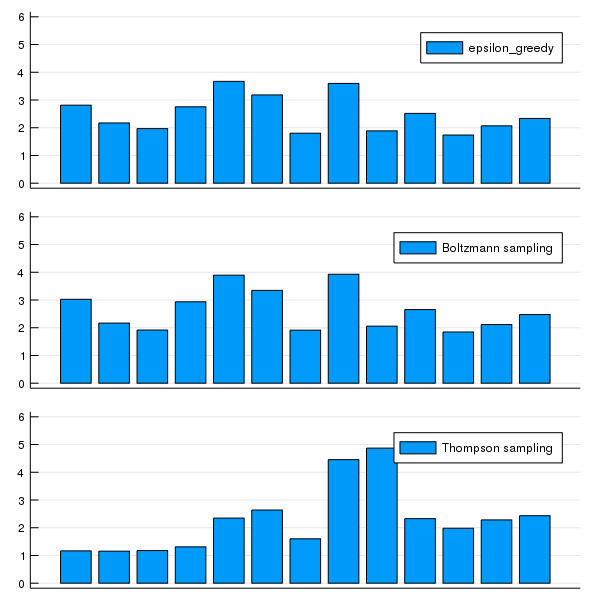
\includegraphics[width=0.8\columnwidth]{mean_max_return_comp.png}
    \caption{The maximum (long-run) ratio of the total return under the MAB algorithm compared to blind guesing for each of our three competitive algorithms. As we can see, while Thompson sampling ended up achieving the highest maximum returns for a few instances, it generally fell behind the more greedy algorithms such as \eg and Boltzmann sampling. If one looks carefully, Boltzmann sampling almost universally slightly outperforms \eg in this case.}
    \label{fig:mean_max_return_comp}
\end{figure}

\section{Conclusion}

Here, I've presented an introduction to the notion of many-armed bandits, which have a rich literature in the mathematics community and have come to be used in machine learning as well. While one can tell, from the often wide gap between the 25th and 75th percentiles of the trials in most of the figures here, that applying MAB algorithms to the gauge selection problem have the risk of a downside and give widely variable results depending on algorithmic choice and problem difficulty, it also provides the opportunity to much more quickly sample the ground state a given number of times than is possible in blind sampling of gauges.

This may prove useful in certain practical applications, though cashing out exactly how useful will require more extensive tests with far larger amounts of data that can truly capture the entire distribution over gauges and precisely pin down the probability density of results per gauge so that one could check the most important concern remaining --- bias in the returned solutions.

The primary reason why one may wish to sample purported ground states many times is to a) gain confidence that one has truly found the ground state and b) to sample a variety of ground states. Without a complete enumeration of ground states and complete statistical characterization of each gauge, answering (b) may well be impossible. Given the extremely conservative nature of our Thompson sampling prior densities, if one wants to achieve (a), then perhaps even despite its lower rate of sampling the ground state, Thompson sampling may well prove preferable. Further work in refining the answers to (a) and (b) are potentially interesting areas for future research effort.

Ultimately, applying MAB algorithms to gauge selection is merely a first step in the long road of trying to learn the map from gauges to probability of success over the space of all instances, which would allow practitioners of quantum annealing to maximally exploit their chosen systems.


% \section{Some examples to get started}

% \subsection{How to include Figures}

% First you have to upload the image file from your computer using the upload link the project menu. Then use the includegraphics command to include it in your document. Use the figure environment and the caption command to add a number and a caption to your figure. See the code for Figure \ref{fig:frog} in this section for an example.

% \begin{figure}
% \centering
% 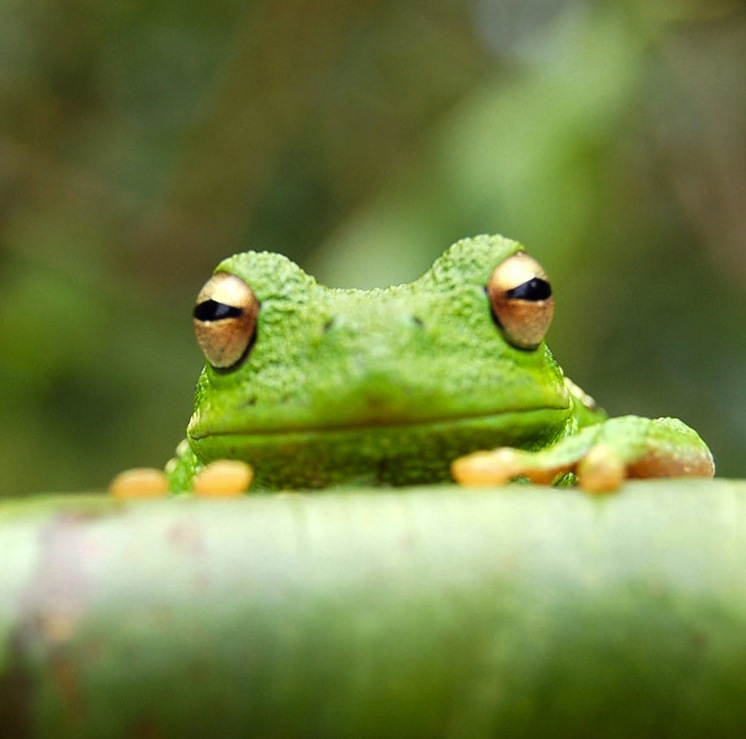
\includegraphics[width=0.3\textwidth]{frog.jpg}
% \caption{\label{fig:frog}This frog was uploaded via the project menu.}
% \end{figure}

% \subsection{How to add Comments}

% Comments can be added to your project by clicking on the comment icon in the toolbar above. % * <john.hammersley@gmail.com> 2016-07-03T09:54:16.211Z:
% %
% % Here's an example comment!
% %
% To reply to a comment, simply click the reply button in the lower right corner of the comment, and you can close them when you're done.

% Comments can also be added to the margins of the compiled PDF using the todo command\todo{Here's a comment in the margin!}, as shown in the example on the right. You can also add inline comments:

% \todo[inline, color=green!40]{This is an inline comment.}

% \subsection{How to add Tables}

% Use the table and tabular commands for basic tables --- see Table~\ref{tab:widgets}, for example. 

% \begin{table}
% \centering
% \begin{tabular}{l|r}
% Item & Quantity \\\hline
% Widgets & 42 \\
% Gadgets & 13
% \end{tabular}
% \caption{\label{tab:widgets}An example table.}
% \end{table}

% \subsection{How to write Mathematics}

% \LaTeX{} is great at typesetting mathematics. Let $X_1, X_2, \ldots, X_n$ be a sequence of independent and identically distributed random variables with $\text{E}[X_i] = \mu$ and $\text{Var}[X_i] = \sigma^2 < \infty$, and let
% \[S_n = \frac{X_1 + X_2 + \cdots + X_n}{n}
%       = \frac{1}{n}\sum_{i}^{n} X_i\]
% denote their mean. Then as $n$ approaches infinity, the random variables $\sqrt{n}(S_n - \mu)$ converge in distribution to a normal $\mathcal{N}(0, \sigma^2)$.


% \subsection{How to create Sections and Subsections}

% Use section and subsections to organize your document. Simply use the section and subsection buttons in the toolbar to create them, and we'll handle all the formatting and numbering automatically.

% \subsection{How to add Lists}

% You can make lists with automatic numbering \dots

% \begin{enumerate}
% \item Like this,
% \item and like this.
% \end{enumerate}
% \dots or bullet points \dots
% \begin{itemize}
% \item Like this,
% \item and like this.
% \end{itemize}

% \subsection{How to add Citations and a References List}

% You can upload a \verb|.bib| file containing your BibTeX entries, created with JabRef; or import your \href{https://www.overleaf.com/blog/184}{Mendeley}, CiteULike or Zotero library as a \verb|.bib| file. You can then cite entries from it, like this: \cite{greenwade93}. Just remember to specify a bibliography style, as well as the filename of the \verb|.bib|.

% You can find a \href{https://www.overleaf.com/help/97-how-to-include-a-bibliography-using-bibtex}{video tutorial here} to learn more about BibTeX.

% We hope you find Overleaf useful, and please let us know if you have any feedback using the help menu above --- or use the contact form at \url{https://www.overleaf.com/contact}!

% \bibliographystyle{alpha}
% \bibliography{refs,sample}

% \end{document}